\documentclass{beamer}

\usepackage{framed}
\usepackage{graphicx}

\begin{document}
	
	\section{Drawing multi-panel categorical plots}
%====================================%
\begin{frame}[fragile]
\frametitle{Seaborn Workshop}
\large
\noindent \textbf{Drawing multi-panel categorical plots}
\begin{itemize}
\item As we mentioned above, there are two ways to draw categorical plots in seaborn. 
\item Similar to the duality in the regression plots, you can either use the functions introduced above, or the higher-level function \texttt{factorplot()}, which combines these functions with a \texttt{FacetGrid()} to add the ability to examine additional categories through the larger structure of the figure.
\end{itemize}

\end{frame}
%====================================%
\begin{frame}[fragile]
	\frametitle{Seaborn Workshop}
	\large
\begin{itemize}
\item While the main options for each plot kind are available either way, the lower-level functions have a bit more flexibility in the kind of inputs they can take.
\item For instance, you can just pass a DataFrame to the data parameter, and the distribution or central tendency of each column in the dataframe will be shown:
\end{itemize}


sns.boxplot(data=iris, orient="h");
\begin{figure}
\centering
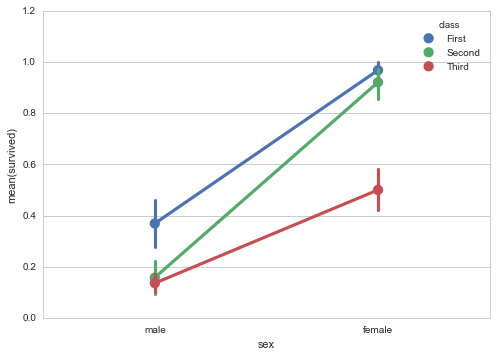
\includegraphics[width=0.7\linewidth]{images/categorical_39_0}
\caption{}
\label{fig:categorical_39_0}
\end{figure}

\end{frame}
%====================================%
\begin{frame}[fragile]
	\frametitle{Seaborn Workshop}
	\large
	
Additionally, these functions accept vectors of Pandas or numpy objects rather than variables in a DataFrame:
\begin{verbatim}
sns.violinplot(x=iris.species, y=iris.sepal_length);
\end{verbatim}

\begin{figure}
	\centering
	\includegraphics[width=0.7\linewidth]{images/categorical_41_0}

\end{figure}
\end{frame}
%====================================%
\begin{frame}[fragile]
	\frametitle{Seaborn Workshop}
	\large
	
To control the size and shape of plots made by the functions discussed above, you must set up the figure yourself using matplotlib commands. Of course, this also means that the plots can happily coexist in a multi-panel figure with other kinds of plots:
\begin{verbatim}
f, ax = plt.subplots(figsize=(7, 3))
sns.countplot(y="deck", data=titanic, color="c");
\end{verbatim}
\begin{figure}
	\centering
	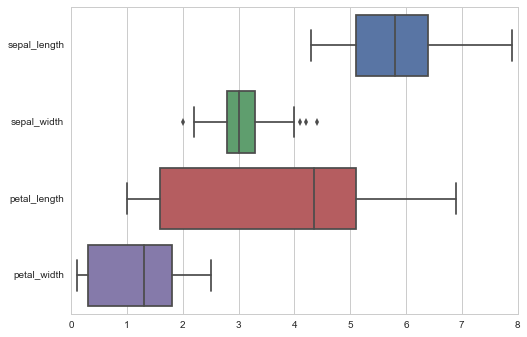
\includegraphics[width=0.7\linewidth]{images/categorical_43_0}
	
\end{figure}
\end{frame}
%====================================%
\begin{frame}[fragile]
	\frametitle{Seaborn Workshop}
	\large
	
The \texttt{factorplot()} function is a higher-level wrapper on these plots that produces a matplotlib figure managed through a FacetGrid:
\begin{verbatim}
sns.factorplot(x="day", y="total_bill", hue="smoker", data=tips);
\end{verbatim}

\begin{figure}
	\centering
	\includegraphics[width=0.7\linewidth]{images/categorical_45_0}
	
\end{figure}
\end{frame}
%====================================%
\begin{frame}[fragile]
	\frametitle{Seaborn Workshop}
	\large
	
By default it uses \texttt{pairplot()}, but the kind parameter lets you chose any of the kinds of plots discussed above:

\begin{verbatim}
sns.factorplot(x="day", y="total_bill", hue="smoker", data=tips, kind="bar");
\end{verbatim}
\begin{figure}
	\centering
	\includegraphics[width=0.7\linewidth]{images/categorical_47_0}
	
\end{figure}
\end{frame}
%====================================%
\begin{frame}[fragile]
	\frametitle{Seaborn Workshop}
	\large
	
The key advantage of \texttt{factorplot()} is that it’s easy to add faceting by additional variables in the DataFrame, such as along the columns:
\begin{verbatim}
sns.factorplot(x="day", y="total_bill", hue="smoker",
               col="time", data=tips, kind="bar");
\end{verbatim}
\begin{figure}
	\centering
	\includegraphics[width=0.7\linewidth]{images/categorical_49_0}
	
\end{figure}
\end{frame}
%====================================%
\begin{frame}[fragile]
	\frametitle{Seaborn Workshop}
	\large
	
Any kind of plot can be drawn. Because of the way FacetGrid works, to change the size and shape of the figure you need to specify the size and aspect arguments, which apply to a single facet:
\begin{verbatim}
sns.factorplot(x="time", y="total_bill", hue="smoker",
               col="day", data=tips, kind="box", size=4, aspect=.5);

\end{verbatim}
\begin{figure}
	\centering
	\includegraphics[width=0.7\linewidth]{images/categorical_51_0}
	
\end{figure}\end{frame}
%====================================%
\begin{frame}[fragile]
	\frametitle{Seaborn Workshop}
	\large
	\begin{itemize}
\item 
Because of the generalized API of the categorical plots, they should be easy to apply to other more complex contexts. 
\item For example, they are easily combined with a PairGrid to show categorical relationships across several different variables:
	\end{itemize}
\end{frame}
%====================================%
\begin{frame}[fragile]
	\frametitle{Seaborn Workshop}
	\large
	\begin{verbatim}
g = sns.PairGrid(tips,
                 x_vars=["smoker", "time", "sex"],
                 y_vars=["total_bill", "tip"],
                 aspect=.75, size=3.5)
g.map(sns.violinplot, palette="pastel");
../_images/categorical_53_0.png
\end{verbatim}
\end{frame}
%====================================%
\end{document}
